\section{Partiella differentialekvationer}

\paragraph{Dirichletvillkor}
Betrakta en differentialekvation som skall lösas på ett domän $\Omega$. Dirichletvillkor är på formen 
\begin{align*}
	u(x, t) = 0, x\in\bound{\Omega}.
\end{align*}

\paragraph{Neumannvillkor}
Betrakta en differentialekvation som skall lösas på ett domän $\Omega$. Neumannvillkor är på formen
\begin{align*}
	n_{i}\del{i}{u(x, t)} = 0, x\in\bound{\Omega},
\end{align*}
där $n$ är normal på $\bound{\Omega}$.

\paragraph{Robinvillkor}
Betrakta en differentialekvation som skall lösas på ett domän $\Omega$. Robinvillkor är på formen
\begin{align*}
	\alpha(x, t)u(x, t) + \beta(x, t)n_{i}\del{i}{u(x, t)} = 0, x\in\bound{\Omega},
\end{align*}
där $n$ är normal på $\bound{\Omega}$.

\paragraph{Homogena och inhomogena grejer}
En differentialekvation på formen
\begin{align*}
	Lu = f
\end{align*}
kallas för homogen om $f = 0$ och inhomogen annars. Vi definierar homogena och inhomogena randvillkor analogt.

\paragraph{Flerdimensionell variant av Sturm-Liouvilles sats}
Problemet
\begin{align*}
	&\laplace{f} = \lambda f, \\
	&f(x) = 0, x\in\bound{\Omega}
\end{align*}
har oändligt många lösningar $f_{n}$ med distinkta egenvärden $\lambda_{n} > 0$ så att lösningarna bildar en fullständig mängd och är ortogonala med inreprodukten
\begin{align*}
	\inprod{f}{g} = \integ[n]{\Omega}{x}{\cc{f}(x)g(x)}.
\end{align*}

För problemet
\begin{align*}
	&\laplace{f} = \lambda f, \\
	&\alpha(x, t)u(x, t) + \beta(x, t)n_{i}\del{i}{u(x, t)} = 0, x\in\bound{\Omega},
\end{align*}
där $n$ är normal på $\bound{\Omega}$, finns det oändligt många ortogonala lösningar med distinkta egenvärden, där dessa bildar en fullständig mängd.

\paragraph{Spektralsatsen}
Låt $A$ vara en självadjungerad operator med diskret spektrum. Då har $A$ oändligt många egenfunktioner. Dessa är ortogonala och bildar en fullständig mängd.

\paragraph{Lösning av PDE:er for dummies}

\begin{figure}[!ht]
	\centering
	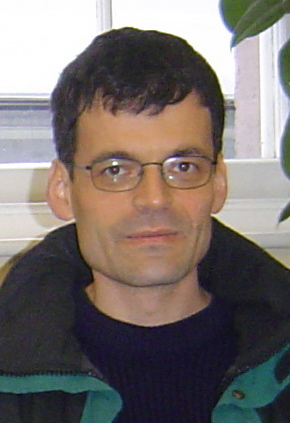
\includegraphics[width = 0.2\textwidth]{./Images/langmann.jpg}
	\caption{Peak fysiker.}
	\label{fig:langmann}
\end{figure}

Fysiker hatar honom. Här kan du läsa hans enkla steg för att göra teoretisk fysik komplett vid att lösa partiella differentialekvationer:
\begin{enumerate}
	\item Hantera inhomogeniteter, så du eventuellt sitter kvar med en homogen ekvation.
	\item Bestäm lösningar till det homogena problemet som passar till randvillkoren. Sturm-Liouvilles sats garanterar att det finns lösningar. Låt den allmänna lösningen vara en linjärkombination av dessa.
	\item Hitta motsvarande lösningar till variabler som inte har randvillkor.
	\item Skriv upp den allmänna lösningen som en linjärkombination av lösningarna du har fått innan.
	\item Välj din linjärkombination så att den passar till initialvillkoren. Sturm-Liouville-teori hjälper även med detta.
\end{enumerate}
Det som följer är sätt att göra dessa olika steg på.

\paragraph{Separationsmetoden}
Separationsmetoden är ett sätt att lösa homogena partiella differentialekvationer på. Dett dåligt sätt, men ändå ett sätt.

Låt $u(x_{1}, \dots, x_{n})$ vara en lösning till $Lu = 0$, där $L$ är en linjär differentialoperator. Separationsmetoden går ut på att göra ansatsen
\begin{align*}
	u = \prod\limits_{i = 1}^{n}X_{i}(x_{i}).
\end{align*}
Denna ansatsen gör förhoppningsvis att differentialekvationen kan skrivas som
\begin{align*}
	\frac{1}{X_{1}}L_{1}X_{1} = \frac{1}{\prod\limits_{i = 1}^{n}X_{i}}L'\prod\limits_{i = 1}^{n}X_{i}.
\end{align*}
Varje sida beror av olika variabler, varför de måste vara lika med en konstant. På detta sättet kan det ursprungliga problemet förhoppningsvis separeras i delproblem som är enkla att lösa.

Den här lösningsmetoden är ej att föredra. Använd heller Sturm-Liouville-teori om du kan.

\subparagraph{Exempel}
\textit{
Lös värmeledningsekvationen $\del{t}u - \alpha\del[2]{x}u = 0,\ u(0, t) = u(L, t) = 0$.
}

För att lösa denna, ansätt $u(x, t) = X(x)T(t)$. Insatt i differentialekvationen ger detta
\begin{align*}
	X\dv{T}{t} - \alpha\dv[2]{X}{x}T = 0,
\end{align*}
som kan separeras till
\begin{align*}
	\frac{1}{\alpha T}\dv{T}{t} = \frac{1}{X}\dv[2]{X}{x}.
\end{align*}
Båda sidor måste vara lika med en konstant $k$. Vi får då två ODE-problem som kan lösas. Lös först $X$-ekvationen, då randvillkoren kommer ge dig ett spektrum av möjliga värden på $k$. För varje sådant $k$ kan du lösa $T$-ekvationen. Lösningen är då en linjärkombination av produkter $XT$, där värje sådant produkt är lösningar av ekvationerna ovan för samma $k$.

\paragraph{Lösning med Sturm-Liouville-teori}
Betrakta ett problem på formen $Lu = 0$, där $L = L_{1} + L_{2}$ och $L_{2}$ är en operator på formen $\frac{1}{w}\dv{x}\left(p\dv{x}\right) + \frac{q}{w}$. Lösning med Sturm-Liouville-teori går ut på att serieutveckla lösningen i egenfunktioner till $L_{2}$, vilket ger ett enklare problem i de återstående variablerna.

Det som är smart med denna metoden är att Sturm-Liouville-teori garanterar att det finns oändligt många sådana egenfunktioner som bildar en fullständig mängd. Vi får även ett sätt att serieutveckla funktioner på genom inreprodukten som kommer från teorin.

Denna lösningsmetoden är helt klart att föredra framför variabelseparation.

\subparagraph{Exempel}
\textit{
Lös diffusionproblemetekvationen $\del{t}u - D\del[2]{x}u = 0,\ u(0, t) = u(L, t) = 0,\ u(x, 0) = u_{0}(x)$.
}

Vi noterar att $-\del[2]{x}{}$ är en operator på formen som beskrivs. Vi kan även hitta sådana egenfunktioner för denna operatorn. Dessa ges av $f_{n}(x) = A_{n}\cos(\sqrt{\lambda_{n}}x) + B_{n}\sin(\sqrt{\lambda_{n}}x)$, där randvillkoren implicerar $A_{n} = 0, \sqrt{\lambda_{n}} = \frac{\pi}{L}n$. Vi gör därmed ansatsen
\begin{align*}
	u(x, t) = \sum\limits_{n = 1}^{\infty}B_{n}(t)\sin(\sqrt{\lambda_{n}}x).
\end{align*}
Insatt i ekvationen ger detta
\begin{align*}
	\del{t}{\sum\limits_{n = 1}^{\infty}B_{n}(t)\sin(\lambda_{n}x)} - D\del[2]{x}{\sum\limits_{n = 1}^{\infty}B_{n}(t)\sin(\lambda_{n}x)}     &= 0, \\
	\sum\limits_{n = 1}^{\infty}\deval{B_{n}}{t}{t}\sin(\lambda_{n}x) + D\sum\limits_{n = 1}^{\infty}B_{n}(t)\lambda_{n}\sin(\sqrt{\lambda_{n}}x) &= 0.
\end{align*}
Man kan slå ihop serierna, och detta implicerar
\begin{align*}
	\dv{B_{n}}{t} + D\lambda_{n}B_{n} = 0.
\end{align*}
För att få ett initialvillkor för $B_{n}$, använd att
\begin{align*}
	u_{0}(x) = \sum\limits_{n = 1}^{\infty}B_{n}(0)\sin(\sqrt{\lambda_{n}}x).
\end{align*}
Sturm-Liouville-teori ger att
\begin{align*}
	u_{0}(x) = \sum\limits_{n = 1}^{\infty}\frac{\inprod{u_{0}}{\sin(\sqrt{\lambda_{n}}x)}}{\inprod{\sin(\sqrt{\lambda_{n}}x)}{\sin(\sqrt{\lambda_{n}}x)}}\sin(\sqrt{\lambda_{n}}x),
\end{align*}
vilket ger initialvillkoret
\begin{align*}
	B_{n}(0) = \frac{\inprod{u_{0}}{\sin(\sqrt{\lambda_{n}}x)}}{\inprod{\sin(\sqrt{\lambda_{n}}x)}{\sin(\sqrt{\lambda_{n}}x)}}
\end{align*}
med inreprodukten
\begin{align*}
	\inprod{f}{g} = \inteval{0}{L}{x}{\cc{f}(x)g(x)}.
\end{align*}

\paragraph{Mer avancerad exempel}
Tillkommer.

\paragraph{Superposition}
Betrakta ett problem på formen $Lu = f$ med olika randvillkor på formen $A_{i}u = g_{i}$. Om problemet är linjärt, kan man skriva lösningen som en summa av olika funktioner, där varje term i summan löser samma problem för fallet alla funktioner $f, g_{i}$ förutom en är lika med $0$.

\subparagraph{Konkretisering}
\textit{
Lös Poissons ekvation $\laplace{u} = f$ för $0\leq x\leq a, 0\leq y\leq b$ med randvillkoren $u(0, y) = g_{1}(y),\ \pdeval{u}{x}{a, y} = g_{2}(y),\ \pdeval{u}{y}{x, 0} = g_{3}(x), u(x, b) = g_{4}(x)$.
}
Lösningen ges av $u = \sum\limits_{i = 1}^{5}u_{i}$, där de olika $u_{i}$ löser
\begin{alignat*}{7}
	\laplace{u_{1}}         &= f,&\ \laplace{u_{2}}         &= 0,       &\        \laplace{u_{3}}         &= 0,&\        \laplace{u_{4}}         &= 0,&\        \laplace{u_{5}}         &= 0,& \\
	u_{1}(0, y)             &= 0,&\ u_{2}(0, y)             &= g_{1}(y),&\ u_{3}(0, y)             &= 0,&\ u_{4}(0, y)             &= 0,&\ u_{5}(0, y)             &= 0,& \\
	\pdeval{u_{1}}{x}{a, y} &= 0,&\ \pdeval{u_{2}}{x}{a, y} &= 0,       &\ \pdeval{u_{3}}{x}{a, y} &= g_{2}(y),&\ \pdeval{u_{4}}{x}{a, y} &= 0,&\ \pdeval{u_{5}}{x}{a, y} &= 0,& \\
	\pdeval{u_{1}}{y}{x, 0} &= 0,&\ \pdeval{u_{2}}{y}{x, 0} &= 0,       &\ \pdeval{u_{3}}{y}{x, 0} &= 0,&\ \pdeval{u_{4}}{y}{x, 0} &= g_{3}(x),&\ \pdeval{u_{5}}{y}{x, 0} &= 0,& \\
	u_{1}(x, b)             &= 0,&\ u_{2}(x, b)             &= 0,       &\ u_{3}(x, b)             &= 0,&\ u_{4}(x, b)             &= 0,&\ u_{5}(x, b)             &= g_{4}(x).&
\end{alignat*}
Nu har vi fått fem enklare problem att lösa, och det kanske går.

\paragraph{Lösningsstrategi för inhomogena problem}
Om man har ett problem med inhomogeniteter i differentialekvationen och/eller villkoren, finns det olika strategier för att lösa detta problemet:
\begin{itemize}
	\item dela upp lösningen i en homogen och partikulär lösning. Den partikulära lösningen fås då vid att gissa en lösning.
	\item flytta inhomogeniteten från villkoren till differentialekvationen, för sen att försöka lösa det.
	\item serieutveckla ekvationen och lösningen, vilket ger ett ODE-problem för basfunktionerna.
\end{itemize}

För att utdypa kring andra metoden, betrakta ekvationen
\begin{align*}
	Lu            &= 0, \\
	Au(\vb{x}, t) &= f(x, t), x\in\bound{\Omega},
\end{align*}
där både $L$ och $A$ är linjära operatorer. Antag att man hittar en funktion $w$ som uppfyller $Aw = f$ på randen, och inför $v = u - w$, där $u$ är en lösning. Denna uppfyller
\begin{align*}
	Lv       &= Lu - Lw = -Lw, \\
	Av(x, t) &= 0, x\in\bound{\Omega}.
\end{align*}

\subparagraph{Exempel}
Tillkommer.

\paragraph{Lösning på oändliga områden}
Betrakta problemet $Lu = f$ på hela $\R^{n}$. För att lösa detta, är det smart att transformera problemet och försöka bryta det ned i minre bitar.

\subparagraph{Exempel}
Tillkommer

\paragraph{Poissonkärnor}
Betrakta en homogen differentialekvation på ett helt reelt rum. Vi vet mha. Fouriertransform att lösningen för ett givet begynnelsesvillkor innebär en faltning av villkoret med någon funktion. Denna funktionen kallas ekvationens Poissonkärna. Den definieras i alla fall för Laplace' ekvation i två dimensioner, så jag väljer denna definitionen. Big whoop, wanna fight about it?

\paragraph{Speglingsmetoder}
Betrakta problemet $Lu = f$ på ett område som ej är oändligt i alla riktningar. Vid att spegla problemet på ett smart sätt kan man utvidga problemet på ett oändligt område, lösa det på det oändliga område och begränsa lösningen till det ursprungliga lösningsdomänet.

\subparagraph{Exempel}
Tillkommer

\paragraph{Greenfunktioner}
För att prata om Greenfunktioner, behöver vi först introducera integralkärnor. Om en linjär operator $L$ på ett intervall $I$ uppfyller
\begin{align*}
	Lf(x) = \integ{I}{y}{K(x, y)f(y)},
\end{align*}
säjs $K$ vara integralkärnan till $L$. Detta kan definieras analogt i flera dimensioner.

Betrakta nu differentialekvationen
\begin{align*}
	Lf = g
\end{align*}
i $d$ dimensioner på området $\Omega$ med homogena randvillkor och begynnelsevillkor. Nu har $L$ givetvis ingen integralkärna, då det är en derivationsoperator. Däremot kan $L^{-1}$ tänkas ha det. Antag vidare att $L^{-1}$ har integralkärnan $G$. Då skulle en partikulärlösning till problemet ovan vara
\begin{align*}
	f = \integ[d]{\Omega}{y}{G(x, y)g(y)}.
\end{align*}
Vi definierar då $G$ att vara Greenfunktionen till $L$.

Hur kan vi hitta Greenfunktioner till en given operator? Vi använder superpositionsprincipen
\begin{align*}
	Lf_{1} = g_{1}, Lf_{2} = g_{2} \implies L(f_{1} + f_{2}) = g_{1} + g_{2}.
\end{align*}
Detta implicerar att om vi kan dela upp $g$ i hanterbara delar och lösa
\begin{align*}
	Lf_{i} = g_{i},
\end{align*}
kan vi hitta Greenfunktionen. Av anledningar som kommer visar sig, väljer vi uppdelningen
\begin{align*}
	Lf_{y}(x) = \delta(x - y), y\in\Omega.
\end{align*}
Låt nu $f_{y}(x) = G(x, y)$. Multiplicera med $g$ på båda sidor och integrera över $y$. Högersidan blir då
\begin{align*}
	\integ[d]{\Omega}{y}{\delta(x - y)g(y)} = g(x).
\end{align*}
Vänstersidan blir
\begin{align*}
	\integ[d]{\Omega}{y}{g(y)LG(x, y)}.
\end{align*}
Eftersom $L$ bara verkar på $x$, kan operatorn $L$ tas ut från integraltecknet, vilket gör vänstersidan till
\begin{align*}
	L\integ[d]{\Omega}{y}{g(y)G(x, y)}.
\end{align*}
Därmed ser vi att
\begin{align*}
	f(x) = \integ[d]{\Omega}{y}{g(y)G(x, y)}
\end{align*}
löser problemet, och det enda som återstår är att lösa differentialekvationen
\begin{align*}
	LG(x, y) = \delta(x - y).
\end{align*}
Denna ekvationen är alltså ett sätt att beräkna Greenfunktioner på.

Den skarpa läsaren märker kanske att inget har specifierats kring randvillkoren. I denna diskussionen förutsätter vi att vi inte behöver bry oss om vad som händer på randen, vilket typiskt är fallet om man betraktar oändliga områden.

Notera att även randvillkor och initialvillkor kommer dyka upp i mer avancerade problem. Att beskriva detta i allmänna fall är svårt, coh ser typiskt olikt ut från problem till problem. Se till konkreta exempel.

\paragraph{Fundamentallösningar}
En fundamentallösning är en Greenfunktion som används för lösningar av ekvationer i hela rummet.

\paragraph{Speglingsmetoder för Greenfunktioner}
Om man vill hitta Greenfunktioner för problem där man behöver betrakta vad som händer på randen, är ett alternativ att använda speglingsmetoder för att utvida problemet till ett oändligt område, där du förhoppningsvis kan hitta en Greenfunktion.

\subparagraph{Exempel}
Tillkommer.